\documentclass{beamer}
 
\usepackage[utf8]{inputenc}
\usepackage{amsmath}
\usepackage{graphicx}
 
 
%Information to be included in the title page:
\title{Degree-based Balanced Clustering for Large-Scale Software Defined Networks}
\author
{
	Talha Ibn Aziz\inst{1} \and 
	Shadman Protik\inst{1} \and
	Md Sakhawat Hossen\inst{1} \and
	Salimur Choudhury\inst{2} \and
	Muhammad Mahbub Alam\inst{1}
}
\institute[IUT]
{
	\inst{1}
	Department of Computer Science and Engineering\\
	Islamic University of Techology\\
	Board Bazar, Gazipur, Bangladesh
	\and
	\inst{2}
	Department of Computer Science\\
	Lakehead University\\
	Thunder Bay, Ontario, Canada
}
\date{IEEE Wireless Communications and Networking Conference, 15-19 April, Marrakech Morocco}
 
 
 
\begin{document}
 
\frame{\titlepage}
 
\begin{frame}
 \frametitle{Table of Contents}
\end{frame}

\begin{frame}
\frametitle{Software Defined Networks (SDNs)}
\begin{itemize}
	\item Software Defined Networks (SDN) decouples the network layer of the traditional protocol stack into the control plane and the data plane
	\item The control plane controls the path selection mechanism and the data plane follows the mechanism to forward data packets.
	\item Devices with high processing capacity called `controllers' communicate with the data plane devices (switches) as per requirement.
	\item The initial design of SDNs included a single controller in a network.
\end{itemize}
\end{frame}

\begin{frame}
\frametitle{Controller Placement Problem (CPP)}
\begin{itemize}
	\item The single controller design gave rise to issues like scalability, reliability - a single point of failure, security, and the formation of a bottle-neck due to overflow of switch-controller queries.
	\item Researches propose a multiple controller approach which introduced a few questions-
	\begin{enumerate}
		\item How many controllers?
		\item Where to place them?
		\item Which switch falls under which controller?
	\end{enumerate}
	\item Several parameters need to be optimized to place multiple controllers, making the solution to the Controller Placement Problem (CPP) NP-Hard.
\end{itemize}
\end{frame}

\begin{frame}
\frametitle{Motivation}
\begin{itemize}
	\item To the best of our knowledge,
	\begin{itemize}
		\item No optimal solution to the CPP has yet been proposed.
		\item The researches done are either exhaustive or work with optimizing a single parameter (latency, reliability, etc.).
	\end{itemize}
	\item Our proposed algorithm Degree-based Balanced Clustering places controllers in polynomial time complexity. DBC simultaneously deals with multiple parameters.
	\item DBC outperforms state-of-the-art controller placement algorithms like Density Based Controller Placement (DBCP), in terms of Flow-Setup Latencies and Load Balancing.
\end{itemize}
\end{frame}

\begin{frame}
\frametitle{Contribution}
DBC is a novel and efficient controller placement algorithm which optimizes the following parameters:
\begin{itemize}
	\item \textbf{Flow setup latency} - The maximum latency incurred to set the path for a new data packet.
	\item \textbf{Route synchronization latency} - Synchronization delay in case of a change in the network due to a link or switch failure.
	\item \textbf{Load of a controller} - The balancing of loads handled by the controllers. The switches are assumed to have identical load.
\end{itemize}
In order to achieve the mentioned goals, DBC forms balanced clusters in terms of both cluster size and inter-switch distances.
\end{frame}

\begin{frame}
\frametitle{Degree-based Balanced Clustering}
Our proposed algorithm performs Controller Placement in three phases.
\begin{enumerate}
	\item \textbf{Cluster Formation} - Group switches for placing a controller (in each group).
	\item \textbf{Controller Selection} - Select one controller among the switches in a group based on some parameters.
	\item \textbf{Selection of optimum number of controllers} - Change the number of controllers and repeat the process to find the optimal configuration.
\end{enumerate}
\end{frame}
\begin{frame}
\frametitle{Cluster Formation}
\begin{enumerate}
	\item Find an approximate cluster radius (hop count).
	\begin{itemize}
		\item Start with a cluster containing only one switch and add switches to the cluster based on average degree.
		\item In each iteration, increment cluster radius by one and add an expected number of nodes to the cluster.
		\item Stop incrementing when the number of nodes exceeds the approximate switch count for a balanced cluster.
	\end{itemize}
	\item Select the switch with highest connectivity as cluster head. We assume that the maximum node degree corresponds to the highest connectivity.
	\item Assign each switch to the nearest cluster head.
\end{enumerate}
\end{frame}

\begin{frame}
\frametitle{Controller Selection}
\begin{itemize}
	\item We select controllers based on weighted-sum of inter-cluster and intra-cluster distances.
	\item Intra-cluster distance for a switch is the average of the distances from the switches of the same cluster.
	\item Inter-cluster distance for a switch is the average of the distances from the switches of the other clusters.
	\item We select the switch with the least weighted-sum in a cluster as the controller of that cluster. Weights can be used to control the extent of inter-cluster or intra-cluster influence while selecting a controller.
\end{itemize}
\end{frame}

\begin{frame}
\frametitle{Optimal number of controller}
\begin{itemize}
	\item Calculate the flow-setup latency for the current network configuration.
	\item Increment the number of controllers and repeat steps 1 (Clustering) and 2 (Controller Selection). Calculate the new route-synchronization latency.
	\begin{itemize}
		\item If the improvement percentage is below a certain threshold, terminate the process.
		\item Otherwise, continue in the same way and increment the number of controllers for another improvement calculation.
	\end{itemize}
\end{itemize}
\end{frame}

\begin{frame}
\frametitle{Experimental Analysis}
\begin{figure}
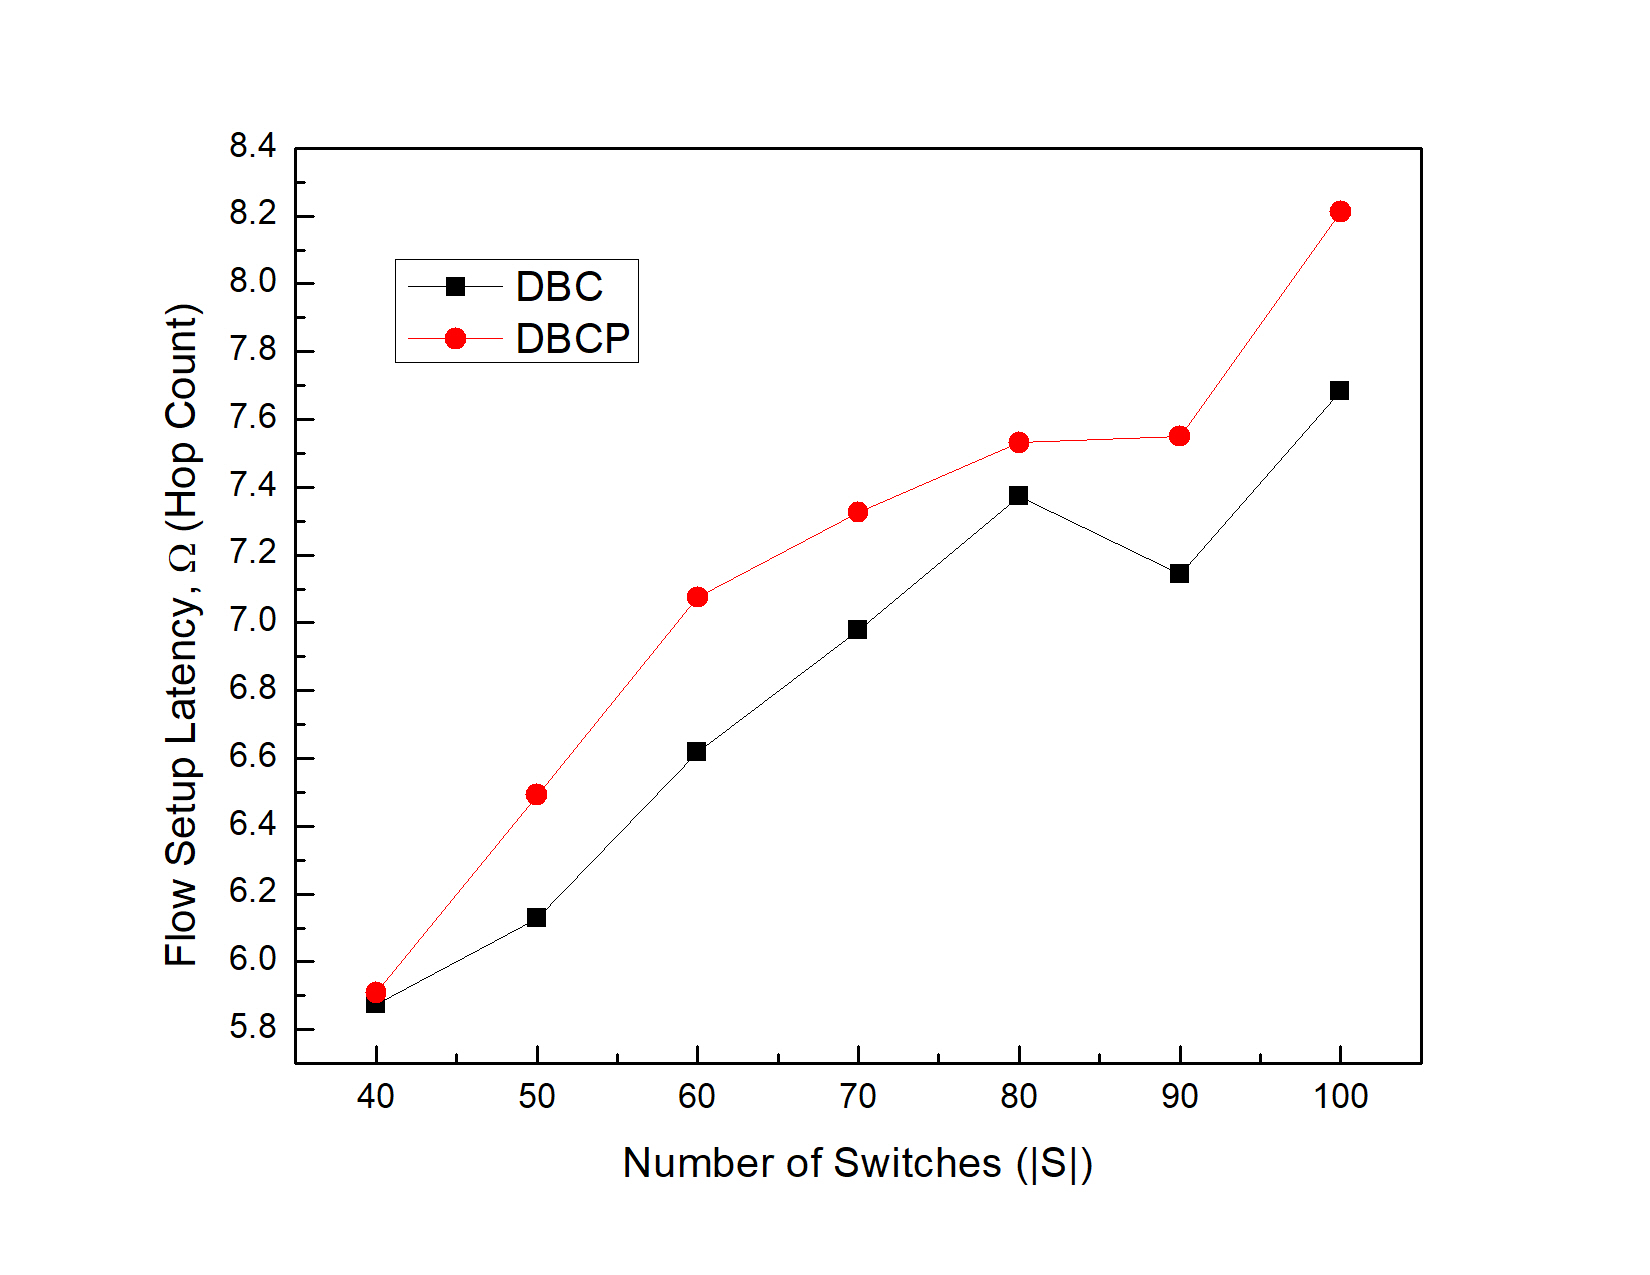
\includegraphics[width=0.8\linewidth]{Figures/dbc_vs_dbcp1.jpg}
\caption{Comparison between DBC and DBCP in terms of Flow Setup Latency for identical numbers of controllers}
\end{figure}
\end{frame}

\begin{frame}
\frametitle{Experimental Analysis}
\begin{figure}
	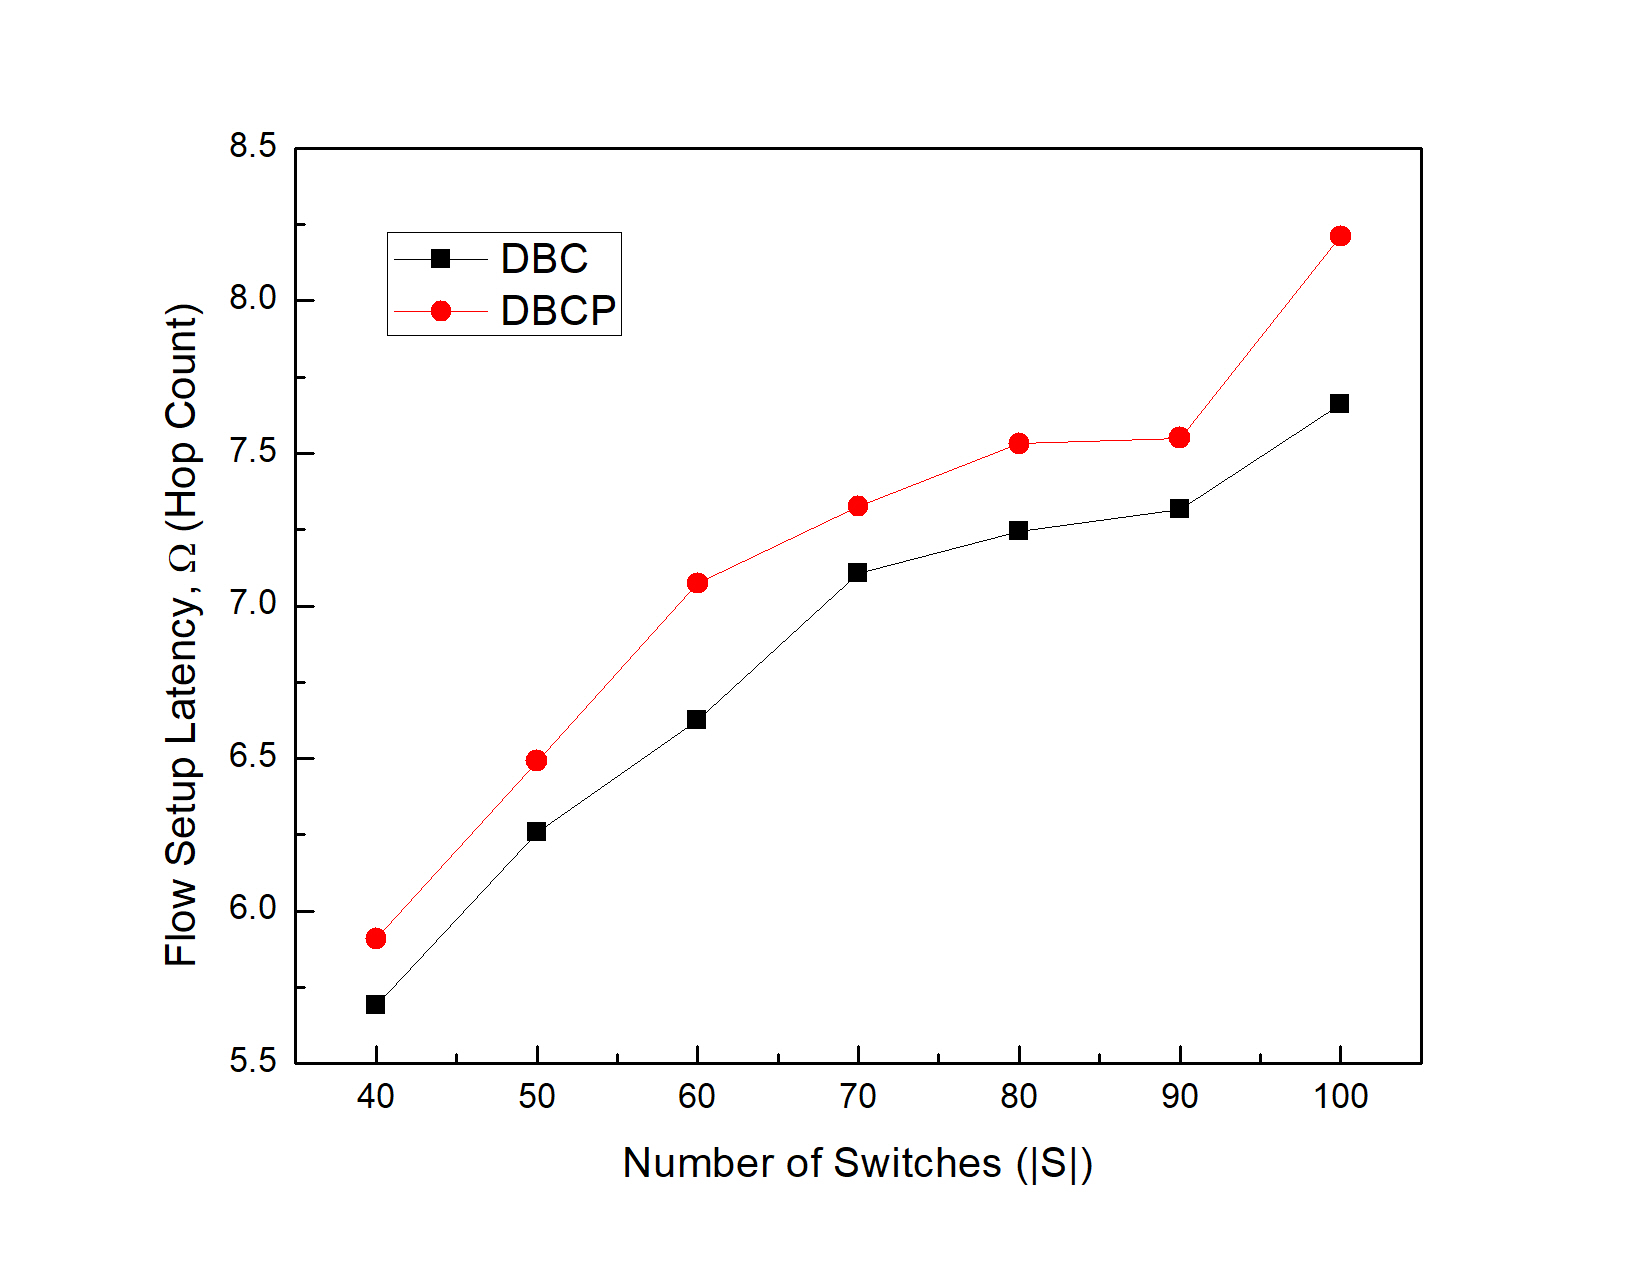
\includegraphics[width=0.8\linewidth]{Figures/dbc_vs_dbcp2.jpg}
	\caption{Comparison between DBC and DBCP in terms of Flow Setup Latency for different numbers of controllers.}
\end{figure}
\end{frame}

\begin{frame}
\frametitle{Experimental Analysis}
\begin{figure}
	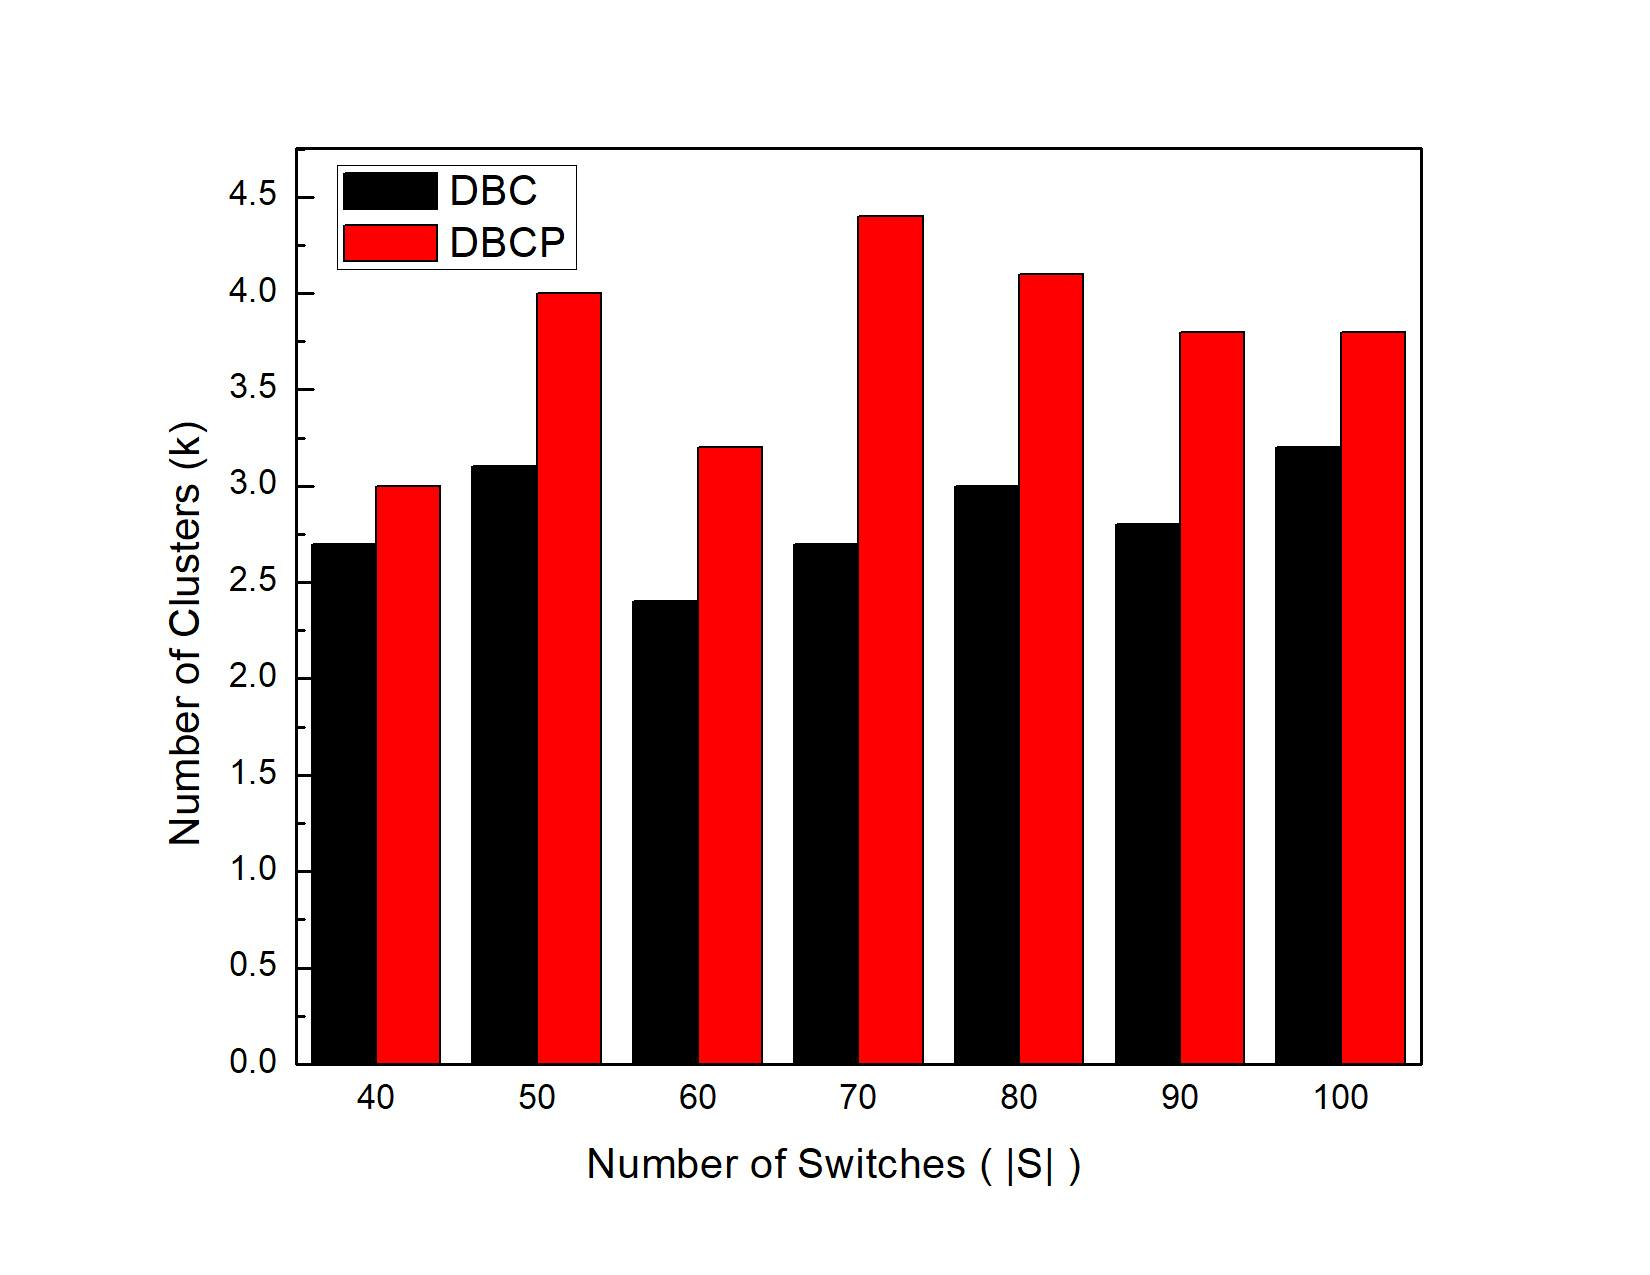
\includegraphics[width=0.8\linewidth]{Figures/bar.jpg}
	\caption{Comparison between DBC and DBCP in terms of Number of Controllers.}
\end{figure}
\end{frame}

\begin{frame}
\frametitle{Experimental Analysis}
\begin{figure}
	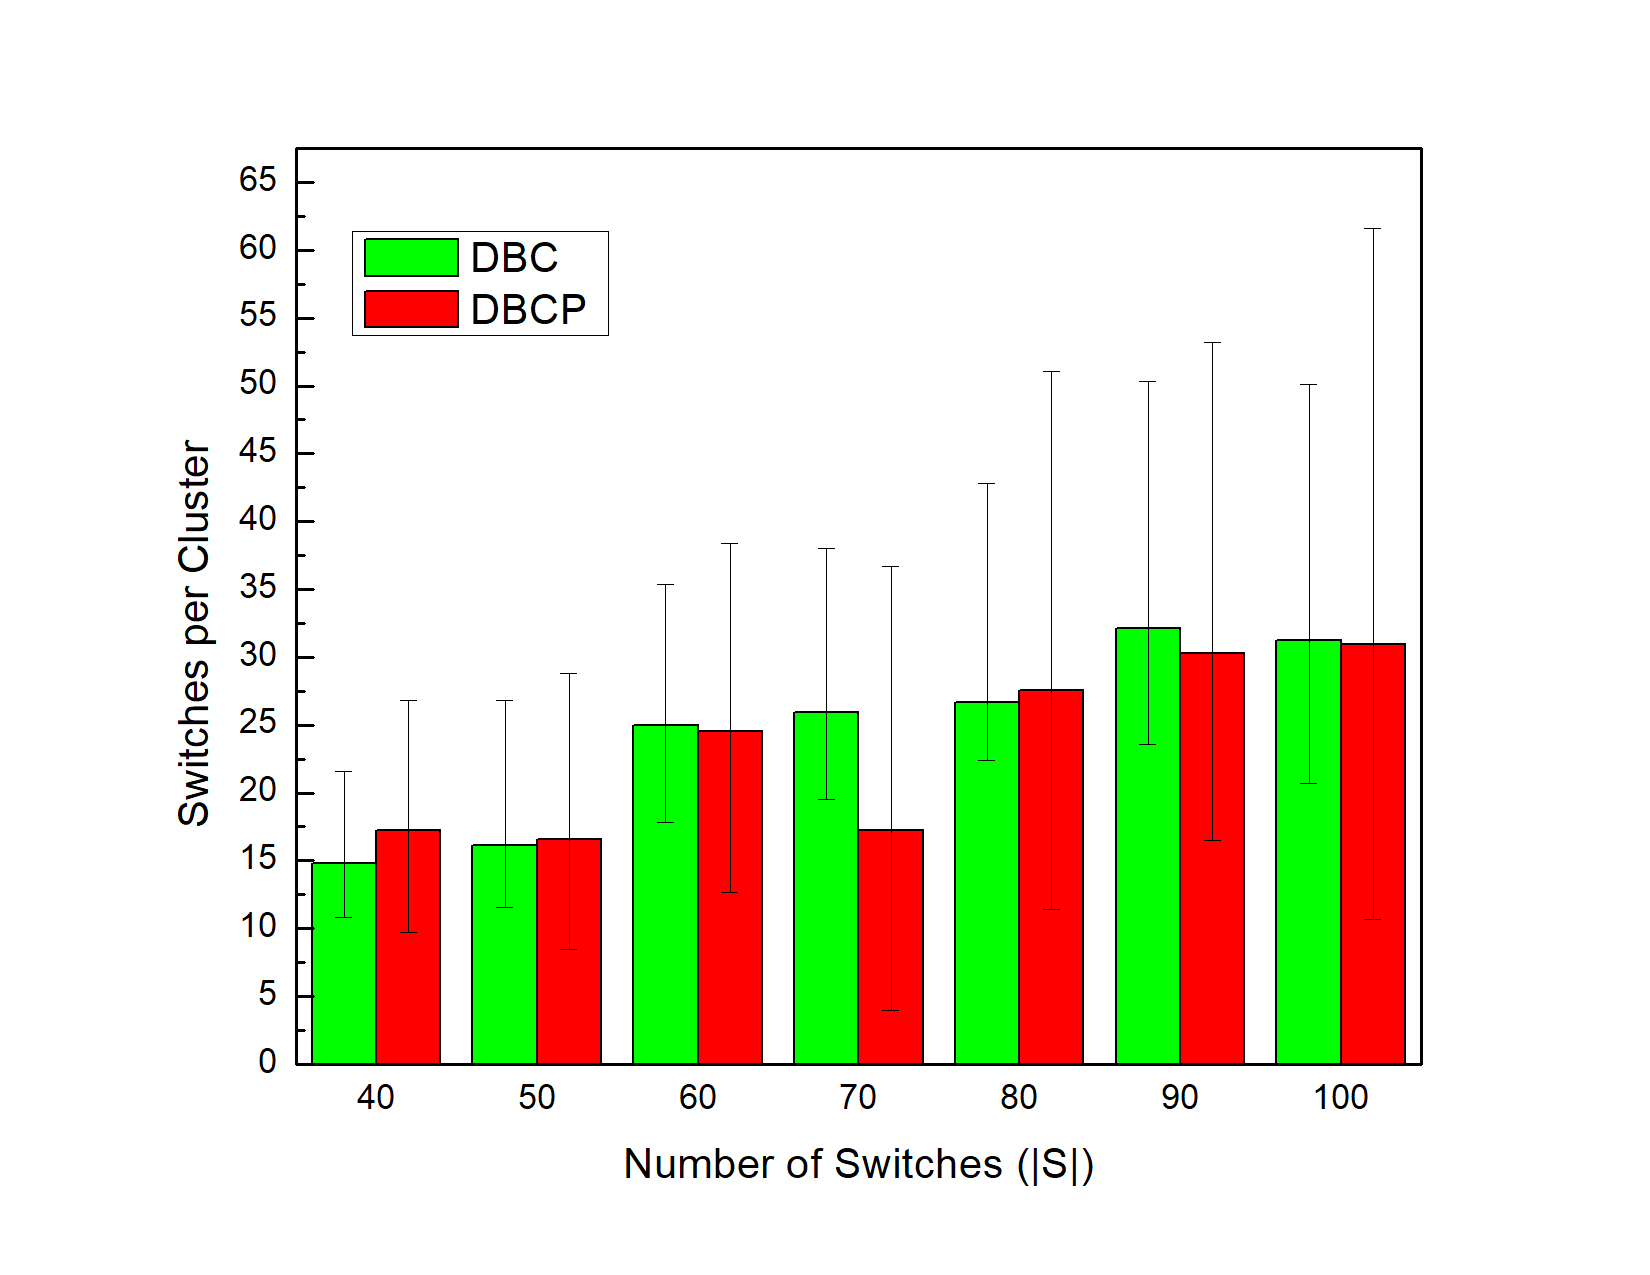
\includegraphics[width=0.8\linewidth]{Figures/loadBalance.jpg}
	\caption{Comparison between DBC and DBCP in terms of maximum, minimum, and average switch distribution.}
\end{figure}
\end{frame}


\begin{frame}
\frametitle{Conclusion}
\begin{itemize}
	\item DBC outperforms DBCP in terms of flow-setup and route-synchronization latencies.
	\item DBC balances the load of the controllers.
	\item Future work may include
	\begin{itemize}
		\item Working with graph representations of networks having variable edge weights (for example - link latencies).
		\item Considering variable controller-processing powers and dynamic switch loads.
	\end{itemize}
\end{itemize}
\end{frame}
 
\end{document}